\documentclass[12pt]{report}
\setlength{\textwidth}{6.3in}
\setlength{\textheight}{9in}
\setlength{\oddsidemargin}{0in}
\setlength{\evensidemargin}{0in}
\setlength{\topmargin}{-.6in}
\linespread{1.2}

% \renewcommand{\labelenumi}{\alph{enumi}}

\newcommand{\be}{\begin{equation}}
\newcommand{\ee}{\end{equation}}
\newcommand{\beq}{\begin{eqnarray}}
\newcommand{\eeq}{\end{eqnarray}}
\newcommand{\beqq}{\begin{eqnarray*}}
\newcommand{\eeqq}{\end{eqnarray*}}
\newcommand{\qed}{\hspace*{\fill}Q.E.D.}  %Use at end of proof
\def\been{\begin{enumerate}}
\def\enen{\end{enumerate}}
\def\beit{\begin{itemize}}
\def\enit{\end{itemize}}

\usepackage{amsfonts}
\usepackage{graphicx}
\usepackage{caption}
\usepackage{subcaption}
\usepackage[toc,page]{appendix}
\usepackage[]{mcode}
\usepackage{listings}
\usepackage{float}
% \hyphenation{ }
\begin{document}

%\begin{Large} \noindent \textbf{Math 412: \\Nicholas von Turkovich} \hfill \textbf{HW IV, due 3/08/16}
%\end{Large}
%\line(1,0){455}

\begin{titlepage}
	\centering
	
{\scshape\LARGE Mathematics 412: Topology \par}
	{\scshape\Large Topological Data Analysis Project\par}
	{\scshape\Large Part 1: Bibliography\par}
	\vspace{1.5cm}
	{\Large TopoCAT : Exploring the Potential Role of TDA in Detecting Lung Cancer\par}
	{\vspace{2cm}}
	
	{\normalsize Brody Kellish, Anirudh Jonnavithula, Nick von Turkovich\par}
	\vspace{1.5cm}
	{\normalsize Thank you to the Duke Mathematics Department for the TDA Tools used in this report\par}
	\vfill


% Bottom of the page
	{\large \today\par}
\end{titlepage}
\newpage

\tableofcontents{}

\part{Background}
\chapter{The Problem}
\section{Idea and Inspiration}
\indent Radiology is one of the most important fields of medicine in terms of early detection and diagnosis of insidious, invasive, and ultimately life-threatening disorders and diseases, especially various forms of cancer. However, the analysis of various types of films (CT, MRI, X-ray, etc.) is a largely subjective process, which draws heavily from the radiologist's history, experience, and own natural biases and tendencies. \\
\indent Modern medical imaging produces large amounts of high-quality image data. Large datasets that combine this image data with official diagnoses are publicly available. A cursory visual inspection of these scans showed obvious visual differences between healthy and ill patients. This delineation suggests that a basic classification algorithm might have some success in analytically determining patient diagnoses. \\
\indent However, such binary classification is not inherently useful on its own - there is a very clear notion of \textit{severity}, that is directly linked to the proliferation of cancerous tissues. This relationship suggests a classic regression problem, in which the characteristics of various forms of medical imagery may be used as as a predictor for patient prognosis.\\
\indent We observe that cancerous tissue in the lung forms \textit{nodules}, which grow and form as the cancer spreads. These nodules are typically small, connected, clusters of distinct tissue, with an underlying structure that appears to generally persist between patients. We hope to apply topological analysis to this image data in order to extract relevant features from these tissue structures, which will be used to develop, train, and test classification and/or regression algorithms.

\section{Hypothesis}
The extraction of topological features from CT scans of patients with and without lung cancer will allow us to train a reliable classification and regression algorithm to accurately and reliably predict:
\begin{itemize}
\item Whether or not this patient has lung cancer (generally).
\item Patient prognosis based on the proliferation, connectivity, and growth of cancerous tissue.
\end{itemize}
\section{Data}

\chapter{The Approach}

\section{Progress So Far}

\par
Some preliminary data processing and feature extraction using the TDA toolkit has yielded some interesting, early results. At the same time, it has uncovered some dilemmas including: how to best down-sample an image to preserve important information while making processing the image practical, what is the best way to generate a point cloud from a down-sampled image, what is the best way to summarize the persistence diagrams of each individual slide in a CT scan and the CT scan as a whole.

\subsection{Visualizing CT Scans in Osirix Lite}

Osirix Lite is the free version of a popular software that is used to visualize and keep track of medical imagery, specifically scans composed of individual images taken over some height function (like CT scans).\newline
\\
Referring to the annotations spreadsheet that accompanies the LIDC-IDRI, a couple subjects were used to get a sense of the visual differences between patients with a large number of nodules and those with relatively "clear" lungs. The two CT scans selected were ID's 321 (25 nodules) and 306 (0 nodules).\newline
\\
Below are cross sections of the lung that illustrate the difference between images of lungs with virtually no growths or nodules and lungs with a large amount of nodules:\newline
\\
\begin{figure}
\centering
\begin{subfigure}{.5\textwidth}
  \centering
  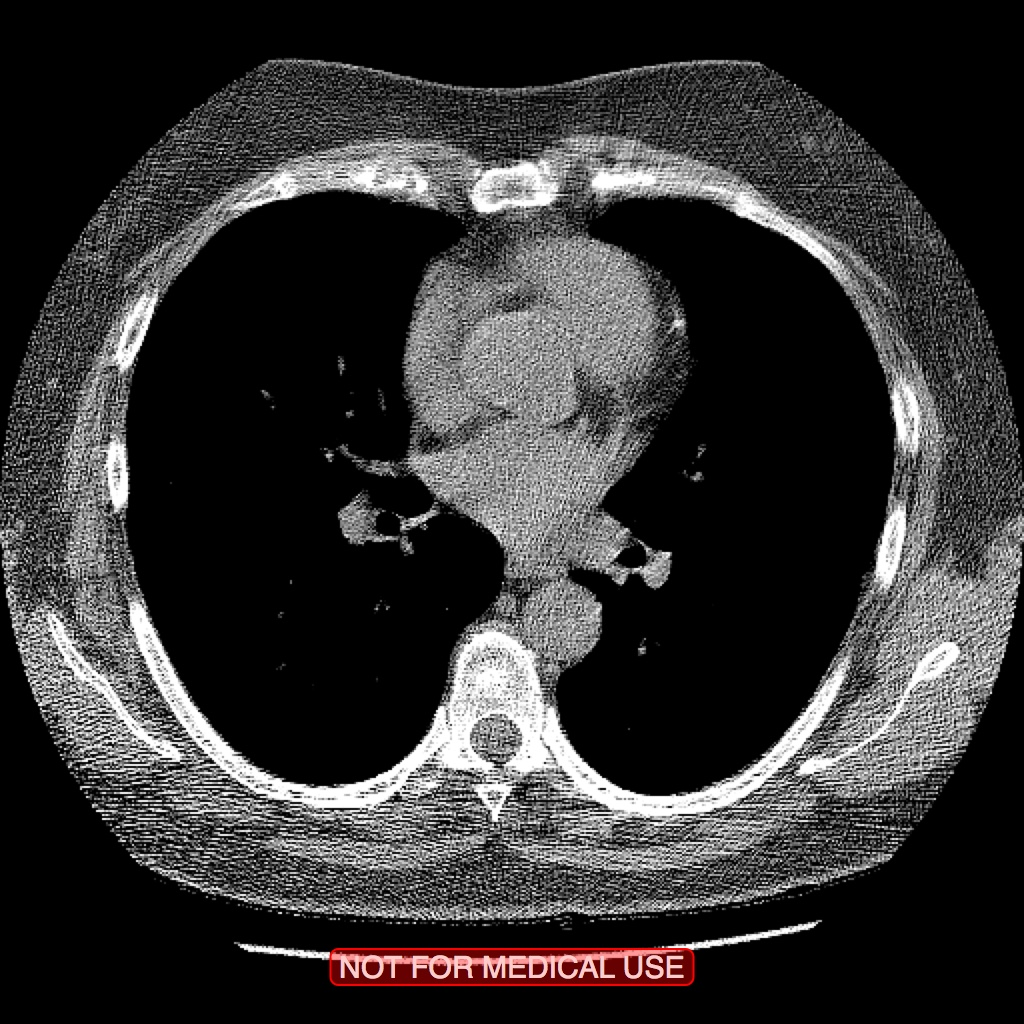
\includegraphics[width=0.8\linewidth]{306example}
  \caption{A Slide from the CT Scan of Patient 306}
  \label{fig:sub1}
\end{subfigure}%
\begin{subfigure}{.5\textwidth}
  \centering
  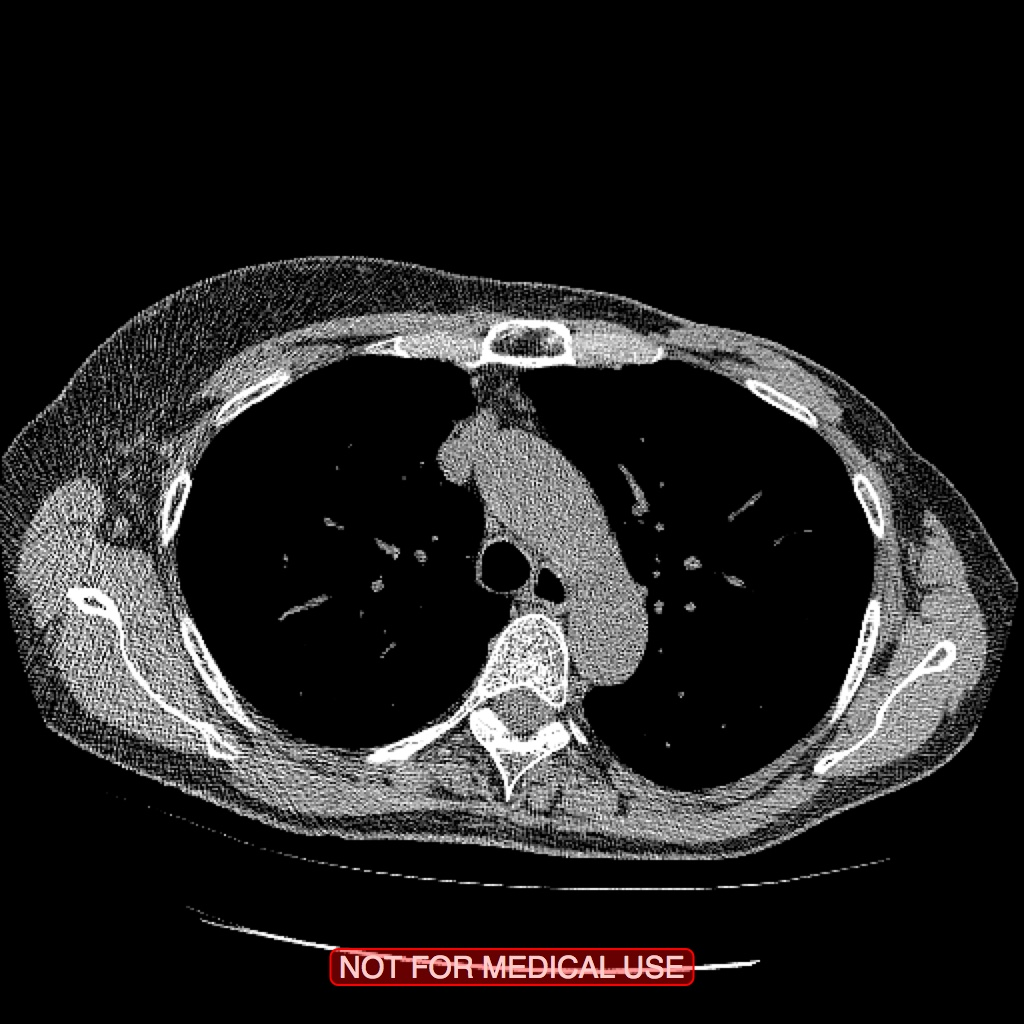
\includegraphics[width=0.8\linewidth]{321example}
  \caption{A Slide from the CT Scan of Patient 321}
  \label{fig:sub2}
\end{subfigure}
\caption{A figure with two subfigures}
\label{fig:test}
\end{figure}\newline
\\
While these cross sections only illustrate the presence of nodules for a particular "height" within the lungs of the two patients, visualizing the images of these cross sections helped to foster an intuition about the topological features of the lungs or images of the lungs. Just from these images, one can see that the number of unconnected components in the image of the patient with a large number of nodules is greater than that of the patient with clear lungs.

\subsection{Filtering Individual Slides of CT Scans by Pixel Intensity}

The first approach to generating persistence diagrams was to triangulate an image based on pixel intensity (see generateS.m in Appendix) values and use that distance matrix to filter the image (testScript.m in Appendix). The findings did not seem to be point to any strong difference between cloudy and clear lungs using this filtration (more work needs to be done on this route to see if it yields anything interesting).\newline
\\
Below are the pre-processed images of the lungs before analysis with rca1mfscm.m.

\begin{figure}[H]
\centering
	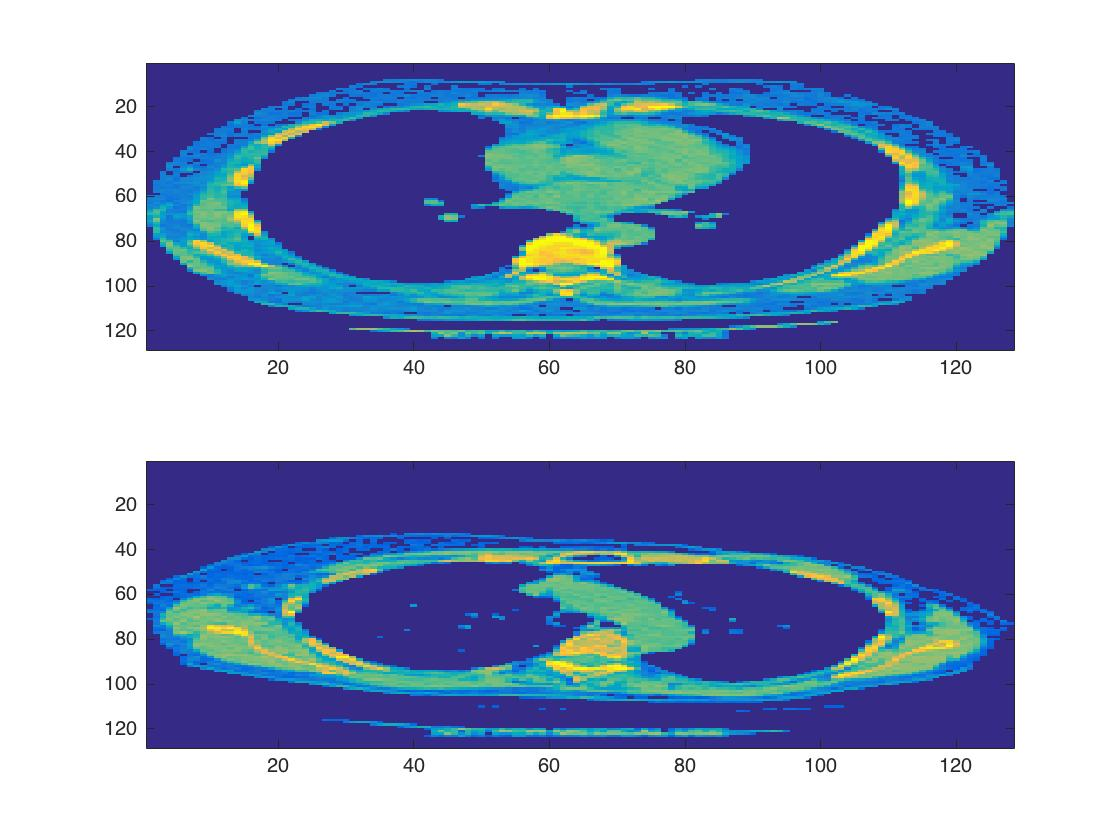
\includegraphics[width=0.8\linewidth]{tSIm.jpg}
	\caption{Post Image Processing: Clear Lung above Cloudy Lung}
\end{figure}\newline
\\
Below are the 0-dimensional and 1-dimensional persistence diagrams for the filtration of the image.
\begin{figure}[H]
\centering
	\includegraphics[width=0.8\linewidth]{0dimpersTs.jpg}
	\caption{$Dgm_0$}
\end{figure}\newline
\\
\begin{figure}[H]
\centering
	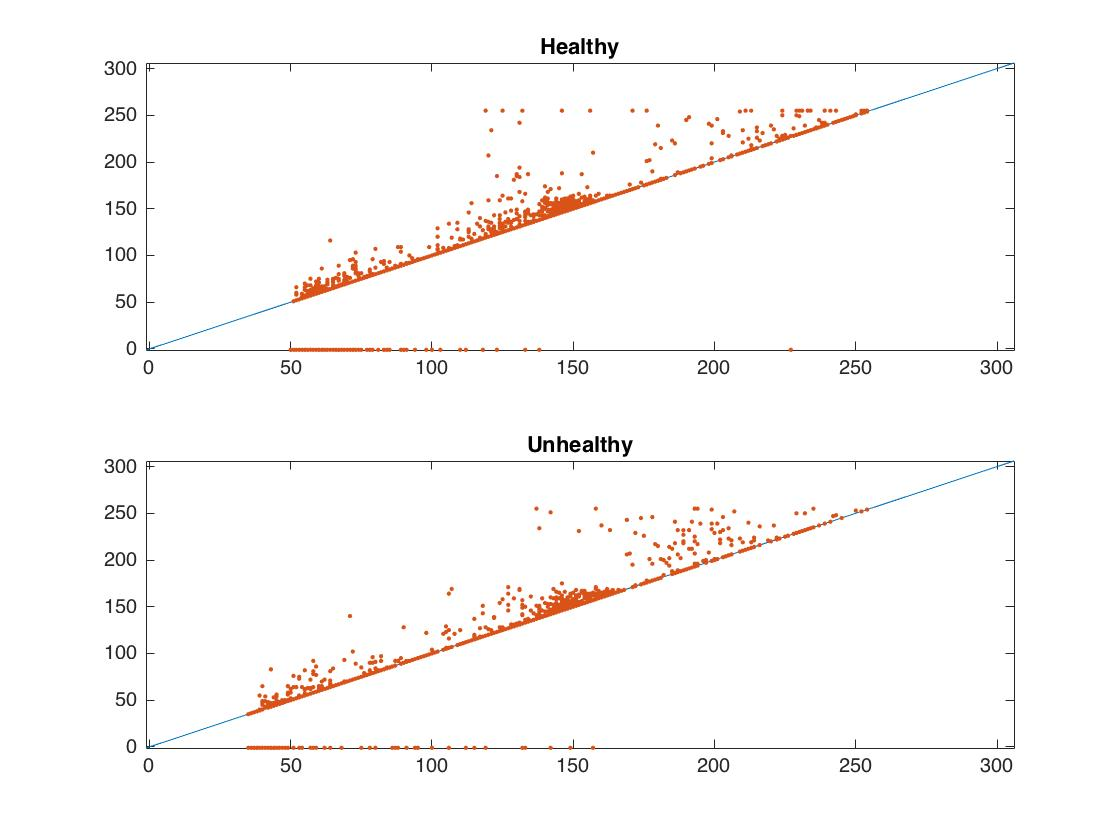
\includegraphics[width=0.8\linewidth]{1dimpersTS.jpg}
	\caption{$Dgm_1$}
\end{figure}\newline
\\

\subsection{Filtering Individual Slides of CT Scans by Generating Point Cloud of Image and Embedding Cloud in $\mathbb{R}^2$}

This approach involved flooring the background of the image and generating points out of the significant pixels (i.e. making the bright pixels in the image vertices). This point cloud was embedded in $\mathbb{R}^2$ and rca1dm.m was used to compute the 0-dimensional and 1-dimensional persistence diagrams (see testScript2.m in Appendix). Below are images detailing the steps of the process: \newline
\\
Below are the original images in grayscale:
\\
\begin{figure}[H]
\centering
	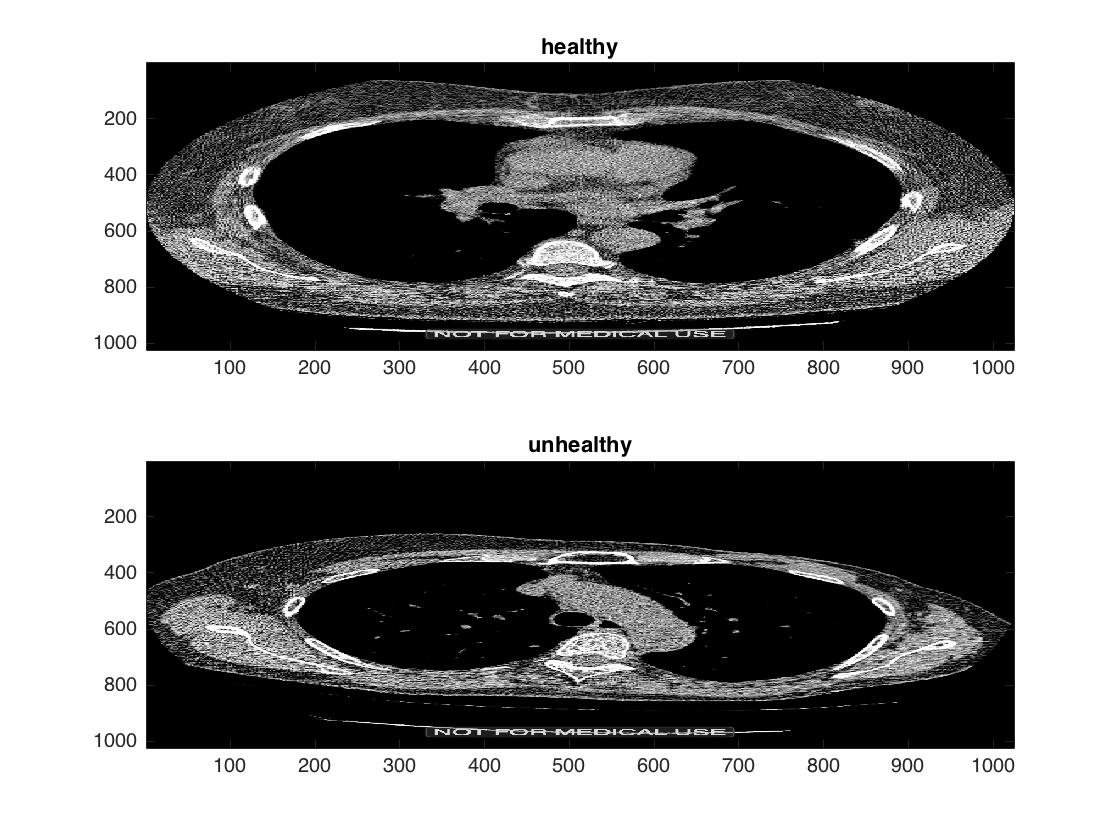
\includegraphics[width=0.8\linewidth]{tS1.jpg}
	\caption{Grayscale Images of the Lungs at a Cross-section for Patients 306 and 321}
\end{figure}\newline
\\
Below are the same images but have been down-sampled by a factor of 0.0625 to make the size of the point cloud manageable:
\\
\begin{figure}[H]
\centering
	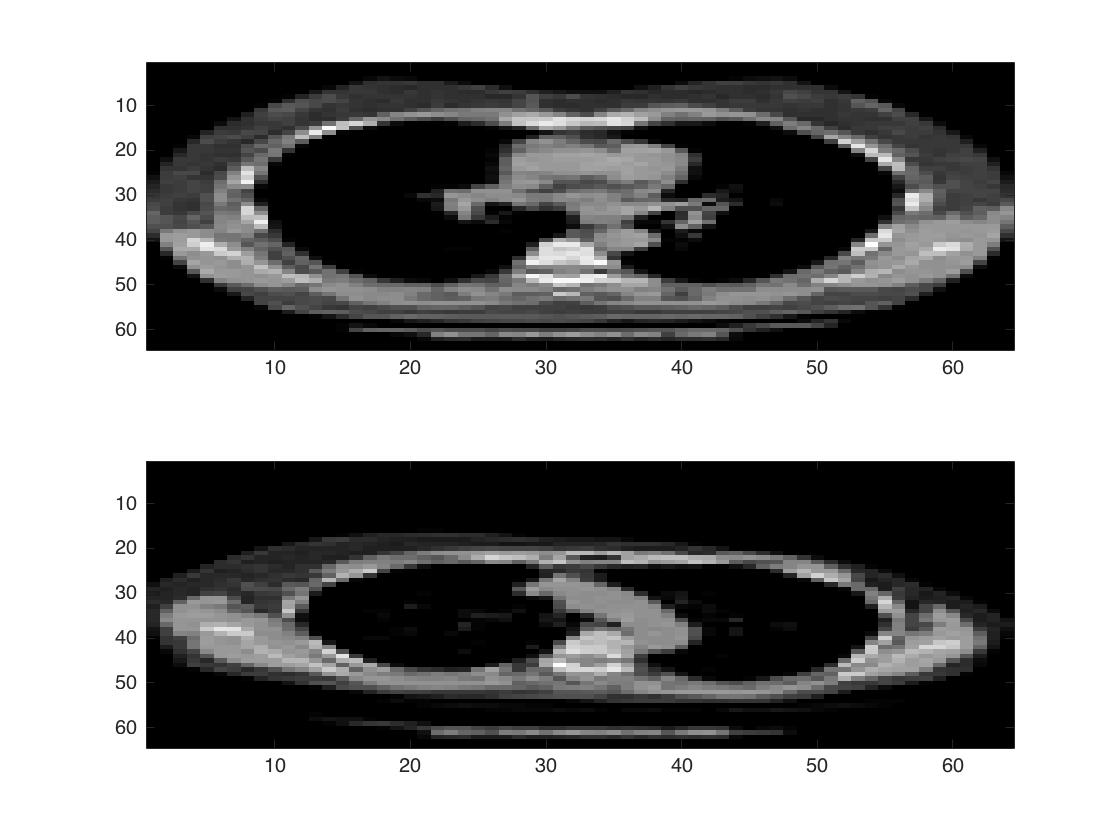
\includegraphics[width=0.8\linewidth]{tS3.jpg}
	\caption{Grayscale, Down-sampled Images}
\end{figure}\newline
\\
Below are the persistence diagrams after running rca1dm.m:
\\
\begin{figure}[H]
\centering
	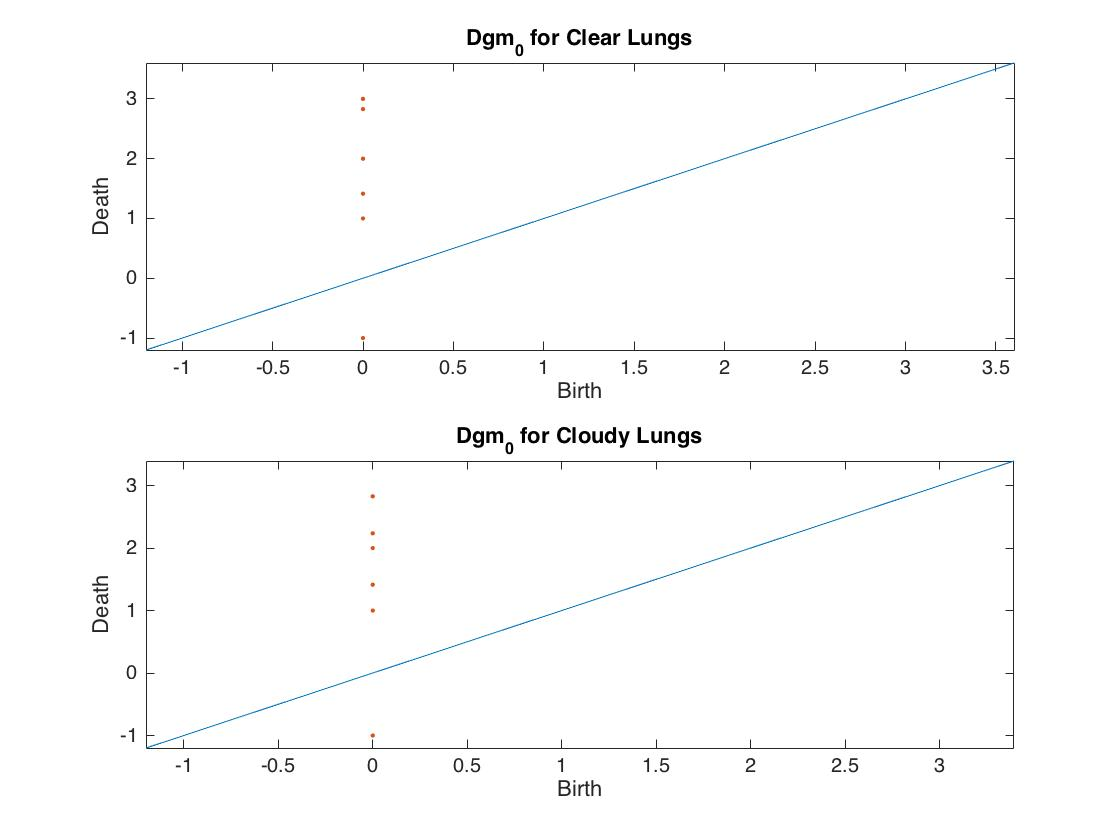
\includegraphics[width=0.8\linewidth]{tSdgm0.jpg}
	\caption{0-Dimensional Persistence Diagram}
\end{figure}\newline
\\
\begin{figure}[H]
\centering
	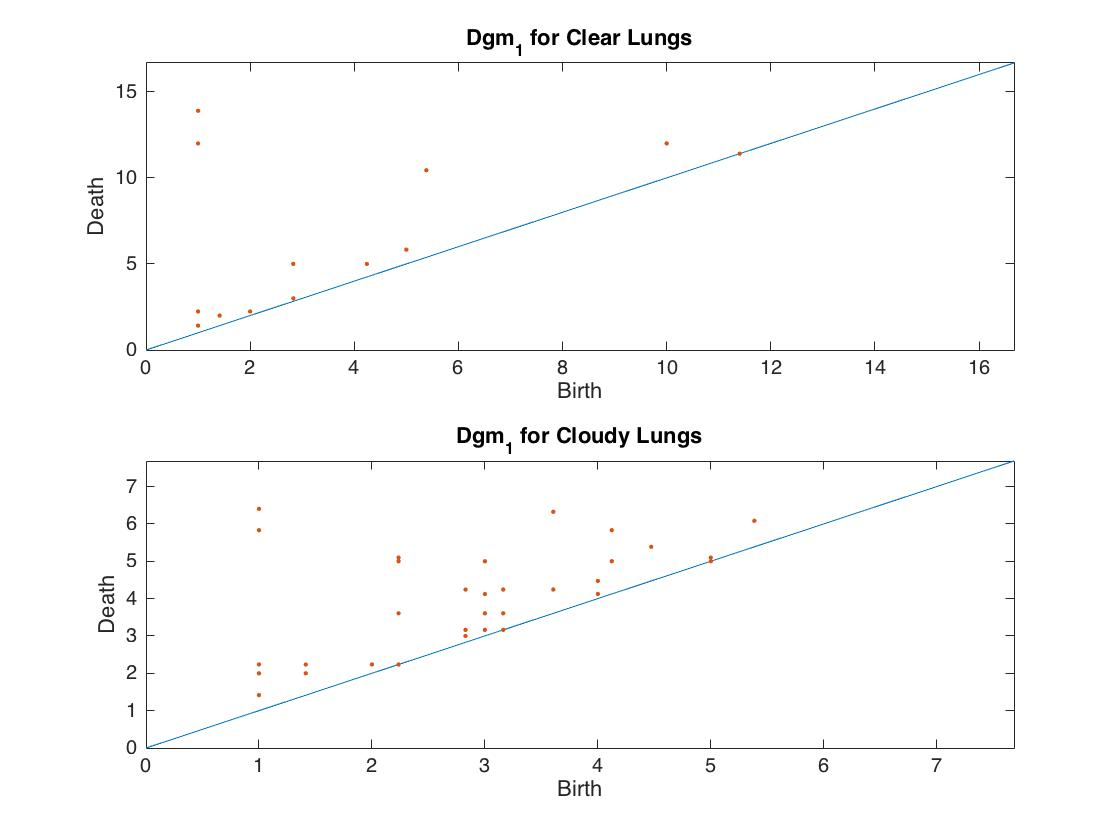
\includegraphics[width=0.8\linewidth]{tSdgm1.jpg}
	\caption{1-Dimensional Persistence Diagram}
\end{figure}\newline

As can be seen in the persistence plots, there seem to be some differences (in this very specific case) between lungs with nodules and lungs without nodules in terms of topological features of their CT scans. This is a very promising start and while we are looking into a few different filtrations to try.\newline
\\
\subsection{Quantifying Topological Features of an Entire Scan from Individual Slides}

Some headway has been made in exploring ways to summarize the information of $N$ slides for a particular CT scan. In the Appendix, testScript3.m and testScript4.m are early attempts at computing persistence using the method of the previous section and tiling up metrics on those values into a vector. For example, by looking at some persistence diagrams of different slides by using the method of 2.1.3, one can see that the "clear" lungs have one or two very persistent 1-cycles and a couple very insignificant 1-cycles. However, for slides of "cloudy" lungs, there is a more even distribution. Therefore, testScript3.m and testScript4.m are concatenating the standard deviation of the 1-dimensional persistence intervals and comparing them for healthy and cloudy lungs. More ways of using the data from each slide will be implemented to see what can maximize the difference between CT scans of patients with clear and cloudy lungs.

\section{Future Directions}

\subsection{Exploring Different Filtrations and Point Cloud Constructions}

\subsection{Quantifying Topological Features of an Entire Scan from Individual Slides (cont.)}

More work needs to be done in exploring how the topological features of one image's point cloud can be combined with the other images in a CT scan to create a vector of information that represents one CT scan (see 2.1.4).

\subsection{Data Storage and Handling}

One tedious but important obstacle is how we are going to:\newline

\begin{enumerate}
	\item Store the ~125 GB of CT scan data
	\item Divide the data into different blocks for processing
	\item Keeping track of each CT scan / how they will be labeled
\end{enumerate}

\subsection{Training and Machine Learning}

The final goal of the project is to train a classifier to identify generally whether a patient has nodes in the lungs or does not as well as a regression model that predicts the degree of tumor proliferation in the lungs based on some metric calculated on the CT scan using our TDA techniques.







\begin{appendices}
\chapter{Appendix}
\section{testScript.m}
\lstinputlisting{/Users/nbv3/Desktop/Math_Projects/topoCAT/TDA/testScript.m}
\section{generateS.m}
\lstinputlisting{/Users/nbv3/Desktop/Math_Projects/topoCAT/TDA/generateS.m}
\section{testScript2.m}
\lstinputlisting{/Users/nbv3/Desktop/Math_Projects/topoCAT/TDA/testScript2.m}
\section{testScript3.m}
\lstinputlisting{/Users/nbv3/Desktop/Math_Projects/topoCAT/TDA/testScript3.m}
\section{testScript4.m}
\lstinputlisting{/Users/nbv3/Desktop/Math_Projects/topoCAT/TDA/testScript4.m}
\end{appendices}


\end{document}